%%%%%%%%%%%%%%%%%%%%%%%%%%%%%%%%%%%%%%%%%%%%%%%%%%%%%%%%%%%%%%%%%%%%%%%%%%%%%%%%%%%%%%%%%%%
%                               Introduction - 3pp
%%%%%%%%%%%%%%%%%%%%%%%%%%%%%%%%%%%%%%%%%%%%%%%%%%%%%%%%%%%%%%%%%%%%%%%%%%%%%%%%%%%%%%%%%%%
\chapter{Introduction}
\label{sec:intro}

\section*{Summary}

\section{Problem}


Even though physical therapy holds a great part of a injured person's rehabilitation, 
it also requires effort from the patient to achieve a full recovery.
In fact, the patient holds great responsibility in each therapy session.
He must be ready to learn about his condition and what types of therapeutic exercises 
to do and how to perform them whenever not being supervised by a therapist (e.g., whenever performing exercises at home).
To be able to exercise alone, a patient must be taught about his body and body 
movements, i.e., he must gain \emph{body awareness}.

A person with an acceptable body awareness has a better knowledge of his body and how to correctly move it when doing exercises or other tasks that involve physical movement.
Therefore, a person is able to improve the overall quality of a given movement and to diminish unnecessary muscle tension, 
by being able to use just the muscles required to accomplish a given task \cite{Singh2014a}.
With relatively low body awareness, it becomes hard for a patient to perform well alone and may 
end up hurting himself. %arranjar exemplos?
Consequently, to help people with low awareness 
execute \textit{prescribed} tasks, it is necessary for them to receive real-time feedback.
This feedback is usually given by a professional, 
but without their presence, it would be desirable for people to receive similar feedback from other sources to maintain a certain quality in the task execution.

\ac{AR} is a technique used to impose digital content on top of the physical world,
giving the user a different perception on the subject in which \ac{AR} is being
applied. This can manipulate the meaning or increase the amount of information available
of the subject being augmented.

\ac{AR} could be a possible solution to overpass the lack of clear feedback sources when no \ac{PT} is present.
It holds great potential in the field of rehabilitation %(and several other serious matters) 
and there are already a variety of tools available to help with the development process of Augmented
Reality applications that interact with the body\cite{Gama2012a}.

If combined with a carefully designed form of feedback for the patient,
\ac{AR} can be of great use in the rehabilitation of a person \cite{Sigrist2013}. The whole 
idea of it is to give more information to a person in a way that it can make 
the assigned task easier to do.
Therefore, the type of feedback given by the \ac{AR} system can have a great influence 
on the outcome of the task being done.\cite{Causo2011}

As above mentioned, the feedback given to a patient helps him to correct mistakes on the performed movements.
Usually, this feedback is given by a therapist while enduring physical therapy, which can be of a visual form (the therapist demonstrating what to do), auditory form (the therapist giving orders to the patient) or physical (the therapist applying physical force to the patient). 
When performing exercises alone, a different approach must be followed on the types of feedback used, making sure that the goals 
are still achieved and the patient performs the exercises correctly.

There are multiple types of feedback, just as there are forms of expression, which means that 
there could be different combinations of feedback that could make a patient understand the task better.
Most of the traditional feedback systems, used for rehabilitation, only use a singular type of feedback,
visual or auditory\cite{Design2005}, being these kind of systems known as \emph{unimodal feedback systems}.

By using multiple types of feedback, we can take advantage of more than one sense on the patient, 
making it possible to give more information without overloading just one sense (e.g., just using visual
cues on a screen can become overwhelming for a patient). A system like the one described is called a 
\emph{multimodal feedback system}, which, by definition, uses various sensory inputs and outputs to achieve the desired task.

\section{Goals}
%qual é o objectivo, qual é a hip que quero provar
%obj e sub-obj

With this work we want to explore the possible benefits of using augmented reality with multimodal 
feedback for guidance in a rehabilitation context.

We plan to analyze several solutions in a variety of fields that rely on feedback for user interaction.
With this analysis we intend to detect the flaws in the current solutions being presented for interaction 
and evaluate which approaches, if combined, could have a chance of improving 
the guidance methods being used with patients.

%After this analysis we will be able to formulate our proposal
%and what it might bring of benefit to this field of rehabilitation.

The document structure is as follows: first, in section \ref{section-related} we will 
explain all the required concepts that are connected to 
this work and overview the state of the art in home rehabilitation systems, giving priority to 
the ones which use some kind of virtual or augmented reality interaction. Also, and most importantly, the feedback strategies used,
not only in these approaches but also in other examples, will be analyzed and compared. 
At the end of this section, an overview will be presented with some conclusions about the current state of the art in multimodal feedback.

Further in the end, in section %\ref{section-approach}
, we will describe our approach with detail, explaining our goals 
while presenting the planned system architecture and evaluation methods to be used.

%The expected contributions to the field of rehabilitation and guiding feedback strategies will also be described.

\section{Approach}


\begin{figure}[!t]
    \begin{center}
        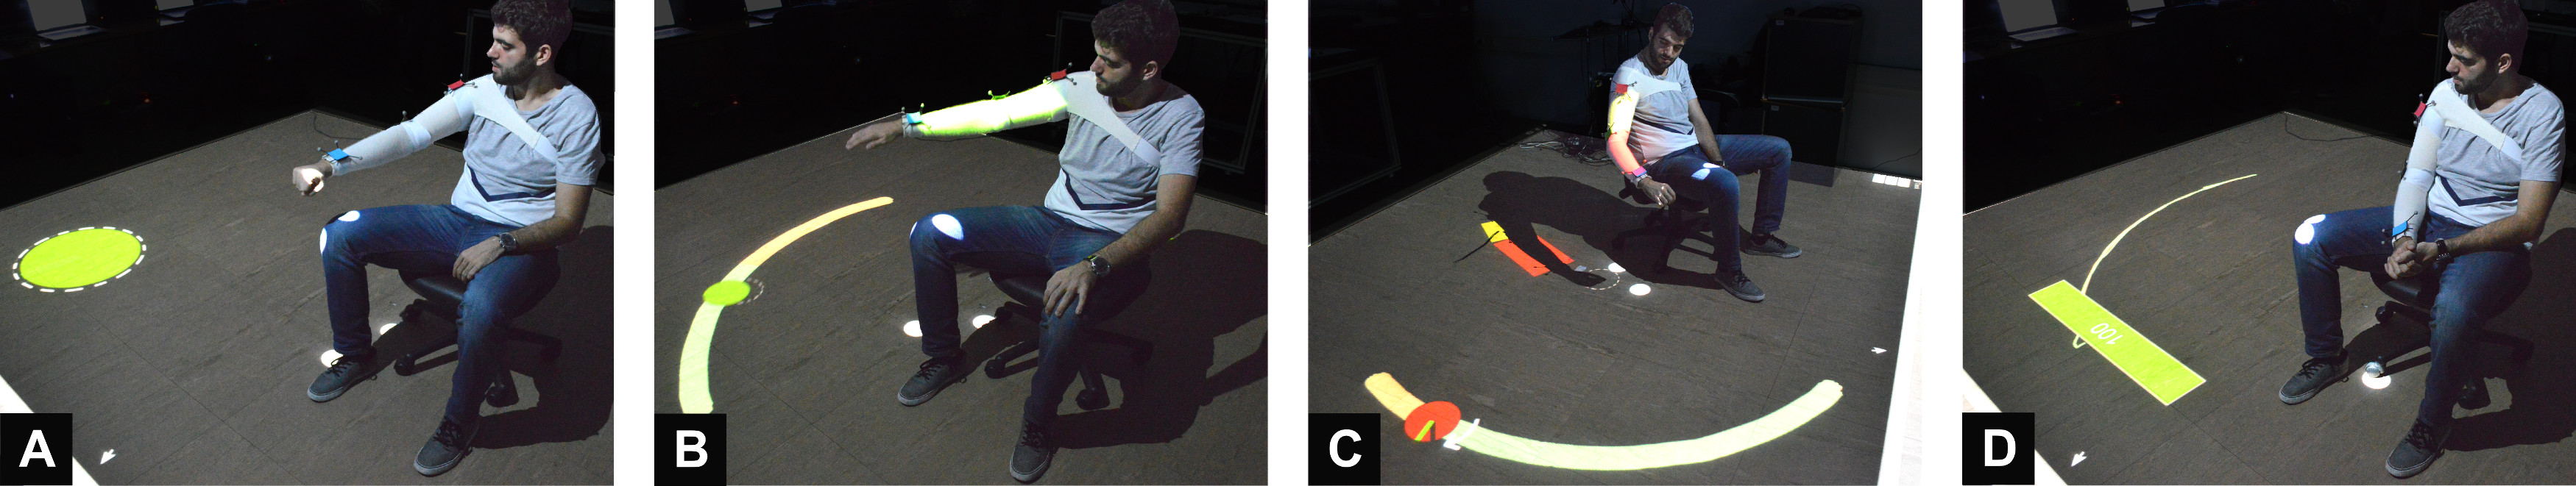
\includegraphics[width=\textwidth]{imgs/impl/teaser.jpg}
    \end{center}
    \caption{SleeveAR addresses new active projection-based strategies for providing user feedback during rehabilitation exercises. a) Initial position. b) Mid-performance. c) Sleeve Feedback. d) Performance review.}
    \label{fig:teaser}
\end{figure}

\section{Contributions}


Studies have already shown that the use of augmented reality feedback enhances the motor learning of an individual \cite{Sigrist2013}.
Aiming to a home rehabilitation process without the presence of a therapist,
the feedback has the responsibility of guiding the patient and correcting him throughout his tasks.

By experimenting on the several forms of feedback that can be used on a patient, we want to evaluate which 
combinations can be useful to specific tasks and how can they complement each other 
in a way that it creates a clear a clear set of instructions for the patient. 
In the end, we want to be able to determine the most appropriate feedback combinations to successfully guide a person through a given movement.
Hence, the aim is to contribute to future augmented reality feedback applications that might need to interact with a user in the clearest possible way.

%The next section presents the state of the art in motor rehabilitation, addressing technological approaches and other important developments.
 

\section{Publications}

\todo{rehab workshop?}

\section{Document Organization}
